\chapter{Resultados}\label{chp:res}

O conjunto de dados, originais e derivados (aqueles criados a partir de dados originais), estão apresentados na tabela X.

\begin{table}[]
\centering
\begin{tabular}{|l|c|c|c|c|}
\hline
Sensor & \multicolumn{4}{c|}{Dado} \\ \hline
 & \multicolumn{4}{l|}{} \\ \hline
Plataforma & Tempo & Mensagem & Tamanho do arquivo \\ \hline
Giroscopio & Taxa de giro em X & Taxa de giro em Y & Taxa de giro em Z &  \\ \hline
Acelerometro & Aceleração em X & Aceleração em Y & Aceleração em Z &  \\ \hline
Pitot & Raw Pitot - Pitot 0 & Pressao Dinamica Ref.- Pitot 0 (virtual) & Velocidade Ref. - Pitot 0 (virtual) &  \\ \hline
Pitot & Raw Pitot - Pitot 1 & Pressao Dinamica Ref.- Pitot 1 (virtual) & Velocidade Ref. - Pitot 1 (virtual) &  \\ \hline
Pitot & Raw Pitot - Pitot 2 & Pressao Dinamica Ref.- Pitot 2 (virtual) & Velocidade Ref. - Pitot 2 (virtual) &  \\ \hline
Pitots & AoA Differential Pressure - Sonda AoA (virtual) 0 & AoA Dynamic Pressure - Sonda AoA 0 (virtual) & AoA - Sonda AoA 0 (virtual) &  \\ \hline
Célula de carga & Raw Cell Data - Celula Horizontal & Forca - Celula Horizontal (virtual) &  &  \\ \hline
Célula de carga & Raw Cell Data - Celula Frontal Direita & Forca - Celula Frontal Direita (virtual) &  &  \\ \hline
Célula de carga & Raw Cell Data - Celula Frontal Esquerda & Forca - Celula Frontal Esquerda (virtual) &  &  \\ \hline
Célula de carga & Raw Cell Data - Celula Traseira Direita & Forca - Celula Traseira Direita (virtual) &  &  \\ \hline
Célula de carga & Raw Cell Data - Celula Traseira Esquerda & Forca - Celula Traseira Esquerda (virtual) &  &  \\ \hline
Células de carga e Pitots & Lift (virtual) & Drag (virtual) & Moment (virtual) & Distance Cp (virtual) \\ \hline
\end{tabular}
\caption{Dados disponíveis no arquivo gerado pela plataforma de aquisição}
\label{tab:all_data_table}
\end{table}

Na imagem X pode ser visto um exemplo dos dados adquiridos durante uma bateria de testes. A gravação dos dados na plataforma ocorre a uma taxa fixa de X Hz, diferente da taxa original de aquisição de cada sensor. 

Isso é feito de modo que todos apresentem uma mesma frequência de ocorrência na plataforma e portanto tenham sempre correspondência nos dados dos outros sensores, facilitando posterior processamento. Neste nivelamento alguns dados, por possuírem frequência de aquisição mais baixa que a de gravação da plataforma, acabam se repetindo até que novos valores estejam disponíveis.

\begin{figure}[!ht]
    \centering
    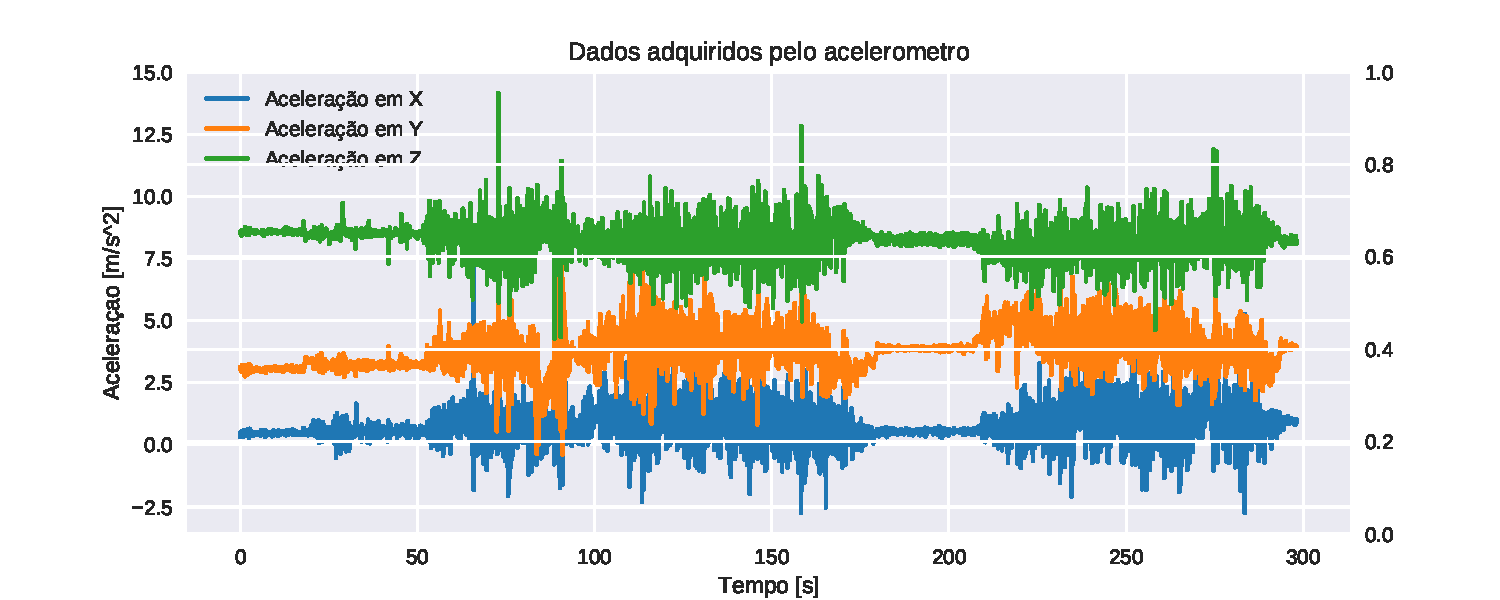
\includegraphics[width=.8\linewidth]{plots/accel_plots.pdf}
    \caption{Exemplo de dados do acelerômetro\cite{autor}.}
    \label{fig:raw_accel_plots}
\end{figure}

\begin{figure}[!ht]
    \centering
    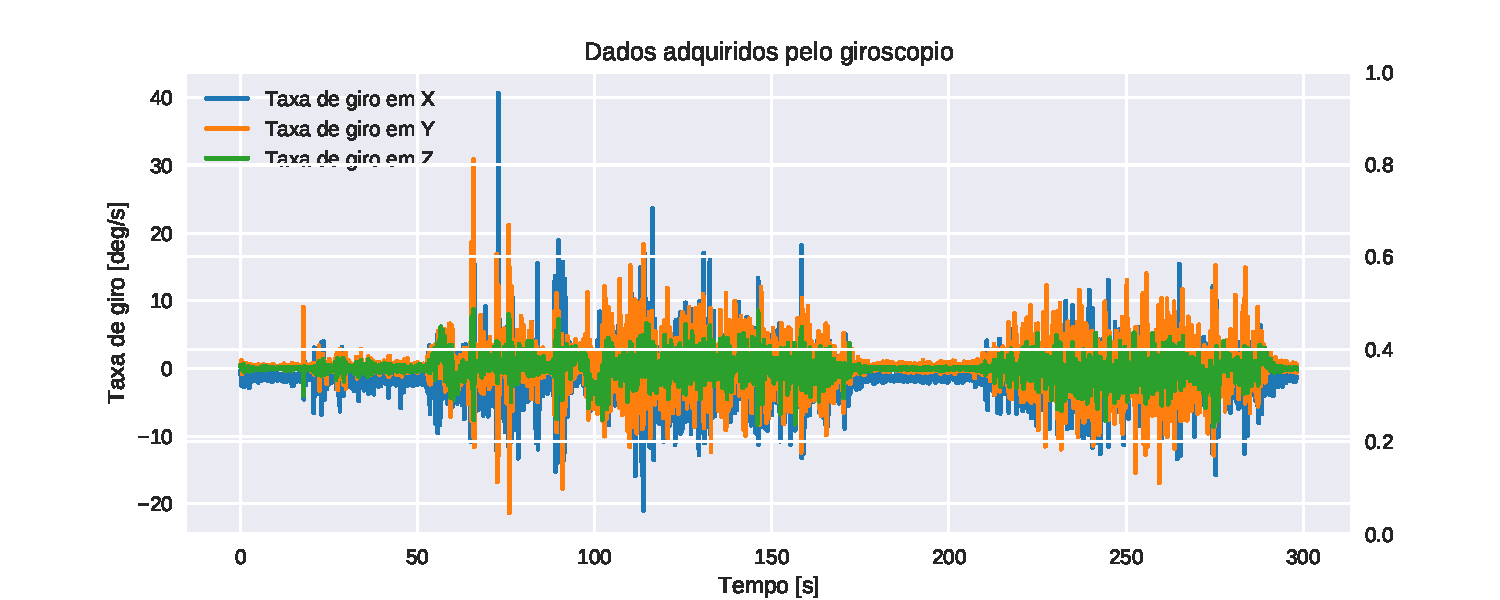
\includegraphics[width=.8\linewidth]{plots/gyro_plots.pdf}
    \caption{Exemplo de dados do giroscópio\cite{autor}.}
    \label{fig:raw_gyro_plots}
\end{figure}

\begin{figure}[!ht]
    \centering
    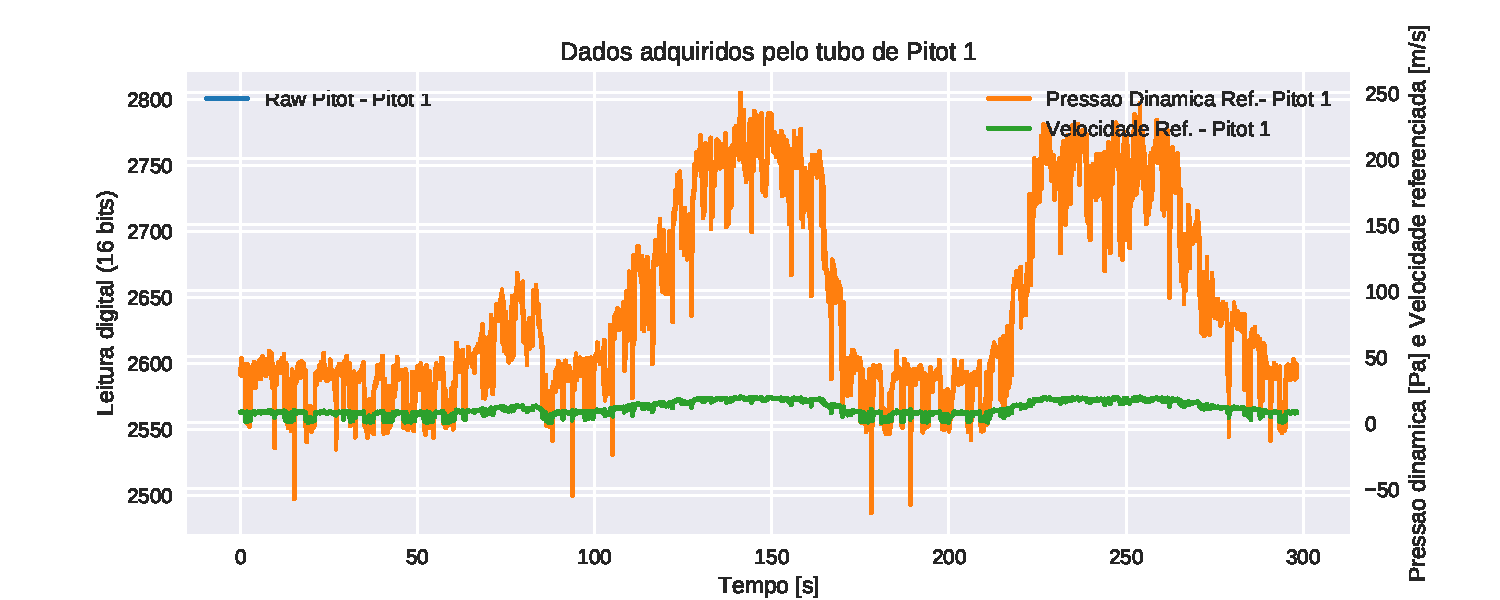
\includegraphics[width=.8\linewidth]{plots/pitot_plots.pdf}
    \caption{Exemplo de dados do Pitot\cite{autor}.}
    \label{fig:raw_pitot_plots}
\end{figure}

\begin{figure}[!ht]
    \centering
    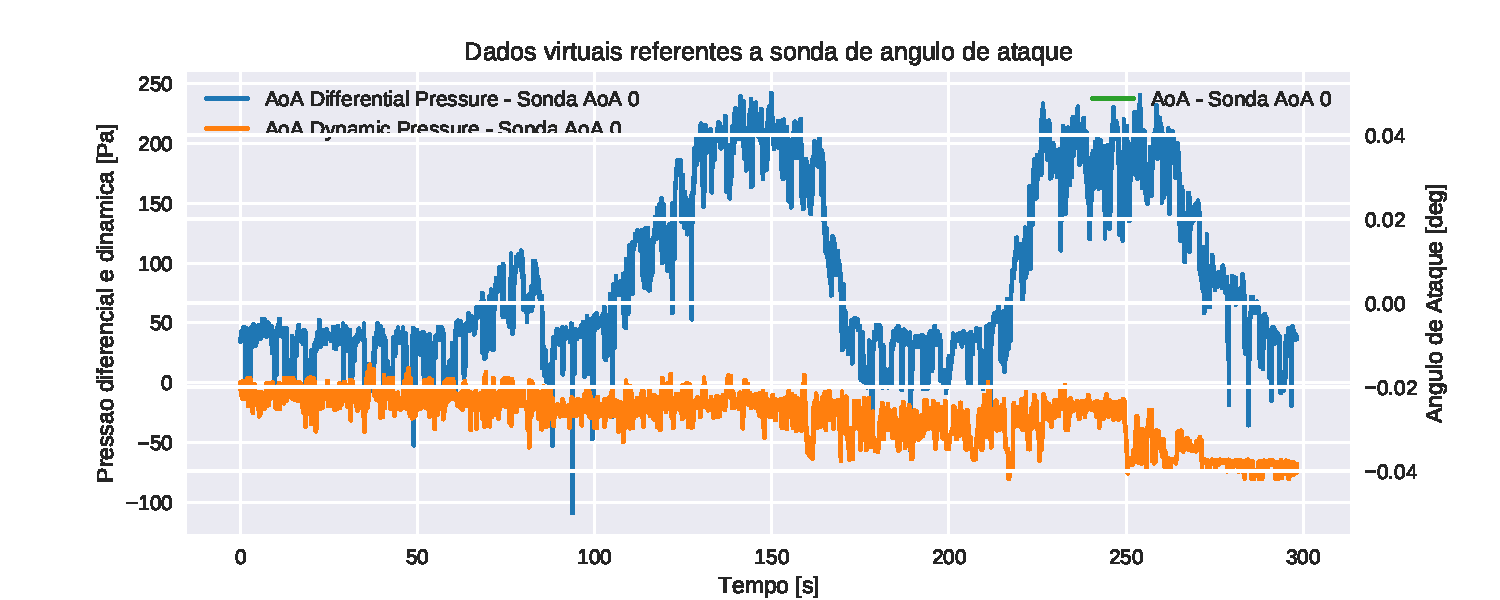
\includegraphics[width=.8\linewidth]{plots/aoa_plots.pdf}
    \caption{Exemplo de dados da sonda de angulo de ataque\cite{autor}.}
    \label{fig:raw_aoa_plots}
\end{figure}

\begin{figure}[!ht]
    \centering
    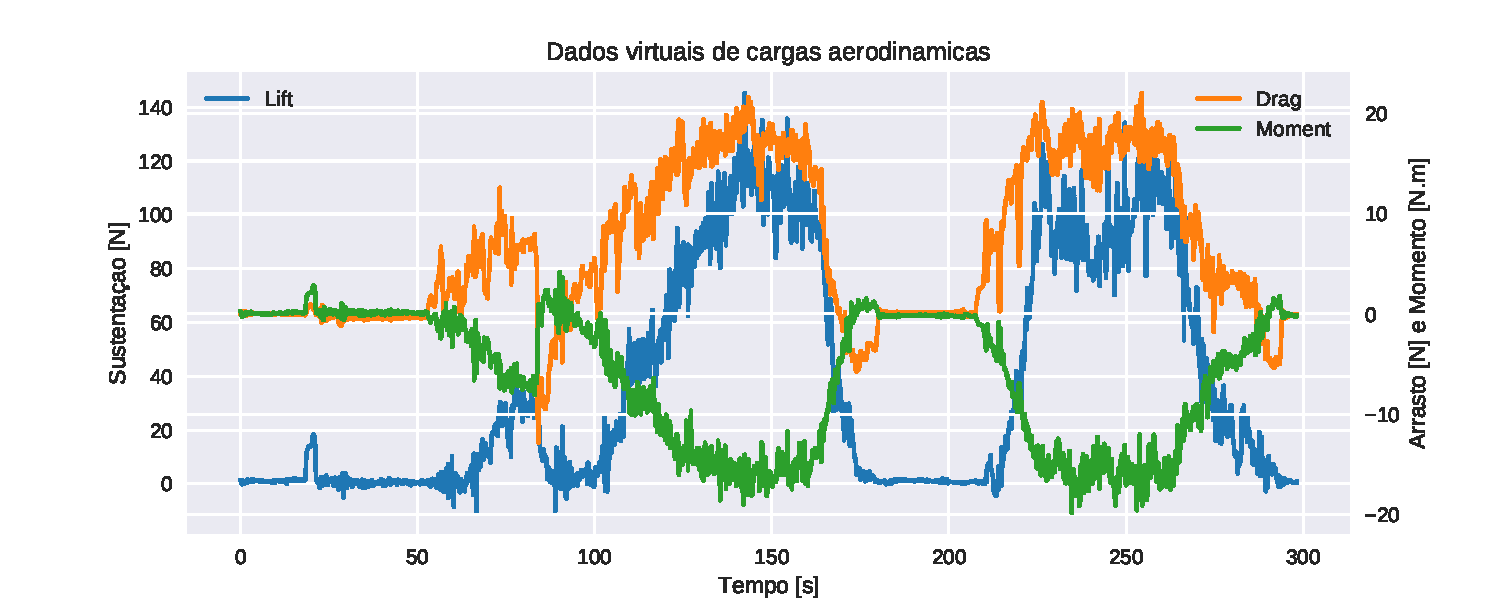
\includegraphics[width=.8\linewidth]{plots/loads_plots.pdf}
    \caption{Exemplo de dados de cargas aerodinâmicas\cite{autor}.}
    \label{fig:raw_load_plots}
\end{figure}

\section{Limpeza, filtragem e redução dos dados}

\subsection{Limpeza de dados}

Dado que o teste foi executado a uma velocidade praticamente constante, o resultado final sera dado para apenas um valor de Reynolds, sendo assim, dados adquiridos que sejam validos mas não estejam próximos ao Reynolds do teste não devem ser utilizados, dado que devem apresentar comportamento aerodinâmico diferente daquele correspondente ao Reynolds desejado[X]. Sendo assim, a primeira limpeza a ser realizada é quanto a faixa de interesse de Reynolds.  Desta forma os dados a serem utilizados para medição serão aqueles correspondentes aos instantes onde foi alcançada velocidade praticamente constante e com um máximo de 10\% de desvio com relação ao Reynolds desejado estipulado.

Para mostrar o resultado desta filtragem usaremos os dados de Sustentação. Os dados originais se encontram na figura \ref{fig:orig_lift_plot} enquanto os dados apos filtragem por faixa de Reynolds se encontram na figura \ref{fig:lift_reynolds_filter} :

\begin{figure}[!ht]
    \centering
    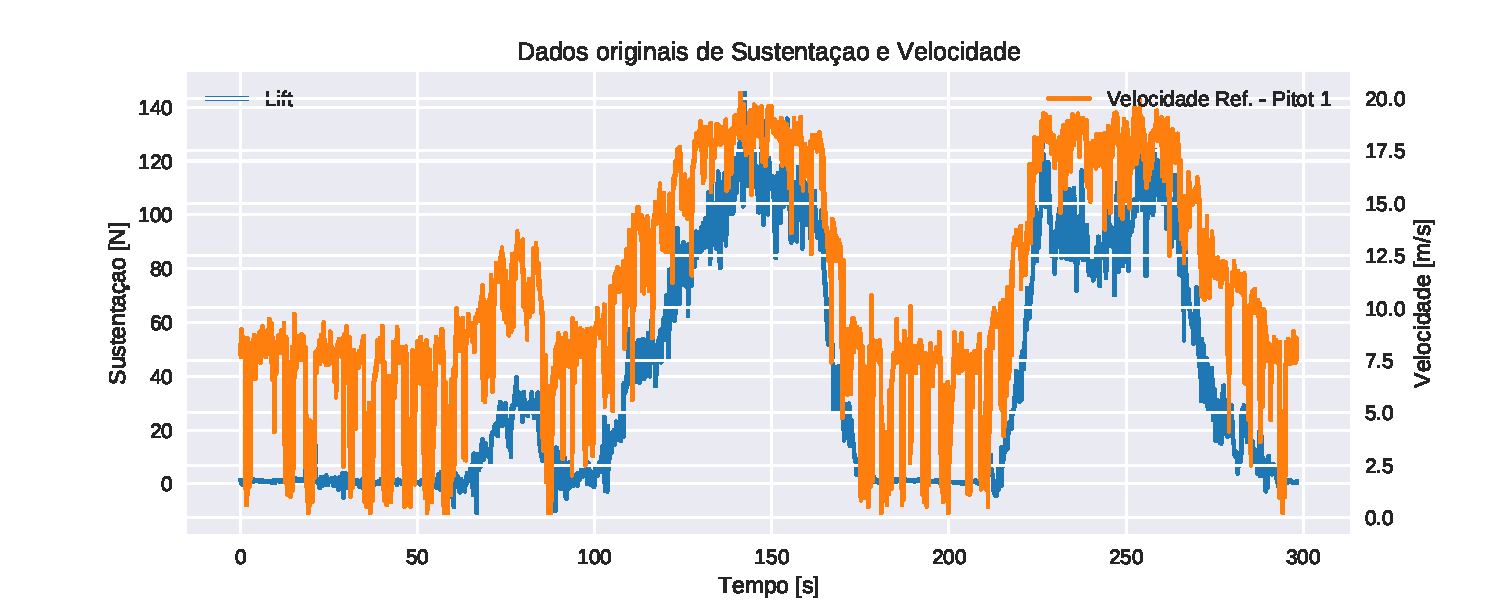
\includegraphics[width=.8\linewidth]{plots/orig_lift_plot.pdf}
    \caption{Dados de sustentação e velocidade originais\cite{autor}.}
    \label{fig:orig_lift_plot}
\end{figure}


\begin{figure}[!ht]
    \centering
    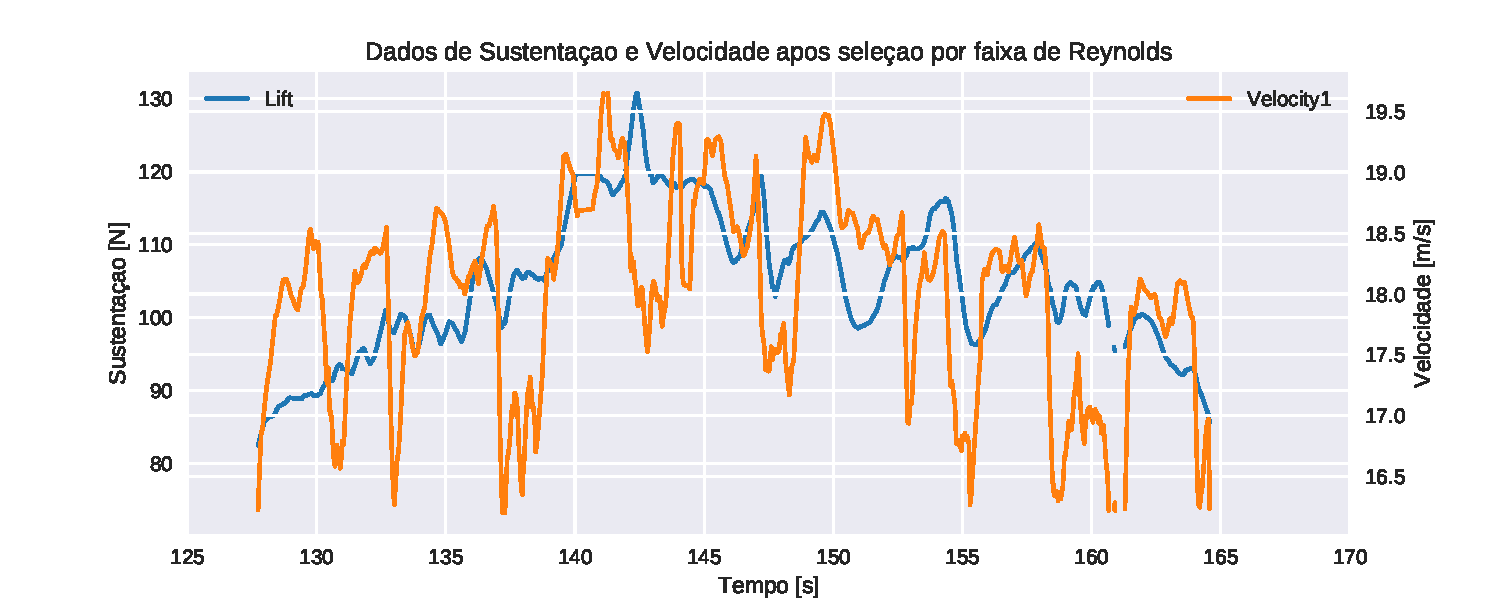
\includegraphics[width=.8\linewidth]{plots/reynolds_lift_plot.pdf}
    \caption{Dados de sustentação e velocidade apos filtragem pela faixa de Reynolds do teste (1o patamar)\cite{autor}.}
    \label{fig:lift_reynolds_filter}
\end{figure}

A premissa principal para o uso dos dados do teste é de que os valores medidos estejam dentro do intervalo de uso dos sensores e de que as acelerações sobre o sistema sejam baixas. O intervalo de uso dos sensores se encontra na tabela X.

\begin{table}[!ht]
    \centering
    
\includegraphics[width=.8\linewidth]{figuras/outras/placeholder.png}
    \caption{TABELA COM ZONA DE USO DE CADA SENSOR\cite{autor}.}
    \label{fig:placeholder}
\end{table}

Apos a seleção por faixa de Reynolds, dados fora da faixa de mediçao dos sensores e dados com aceleração em X, Y ou Z maior que 0.5g foram também descartados.

\subsection{Filtragem}

Apos a limpeza dos dados, onde foram removidos aqueles que estavam fora da zona de interesse, buscou-se avaliar a filtragem do sinal, visando aumentar a relação sinal-ruido. Para isto foi realizada uma analise FFT[X] nos dados de carga, velocidade e aceleração.

\begin{figure}[!ht]
    \centering
    
\includegraphics[width=.8\linewidth]{figuras/outras/placeholder.png}
    \caption{ANALISES FFT\cite{autor}.}
    \label{fig:fft_analysis}
\end{figure}

A partir do resultado das analises foram dimensionados filtros do tipo passa-baixa para a remoção dos ruídos de alta frequência em cada um dos dados[X]. As frequencias de corte para cada dado se encontram na tabela X. Os resultados apos filtragem se encontram na figura X.

\begin{table}[!ht]
    \centering
    
\includegraphics[width=.8\linewidth]{figuras/outras/placeholder.png}
    \caption{TABELA COM FREQUENCIA DE CORTE DE CADA DADO\cite{autor}.}
    \label{tab:cut_frequency_values}
\end{table}

\begin{figure}[!ht]
    \centering
    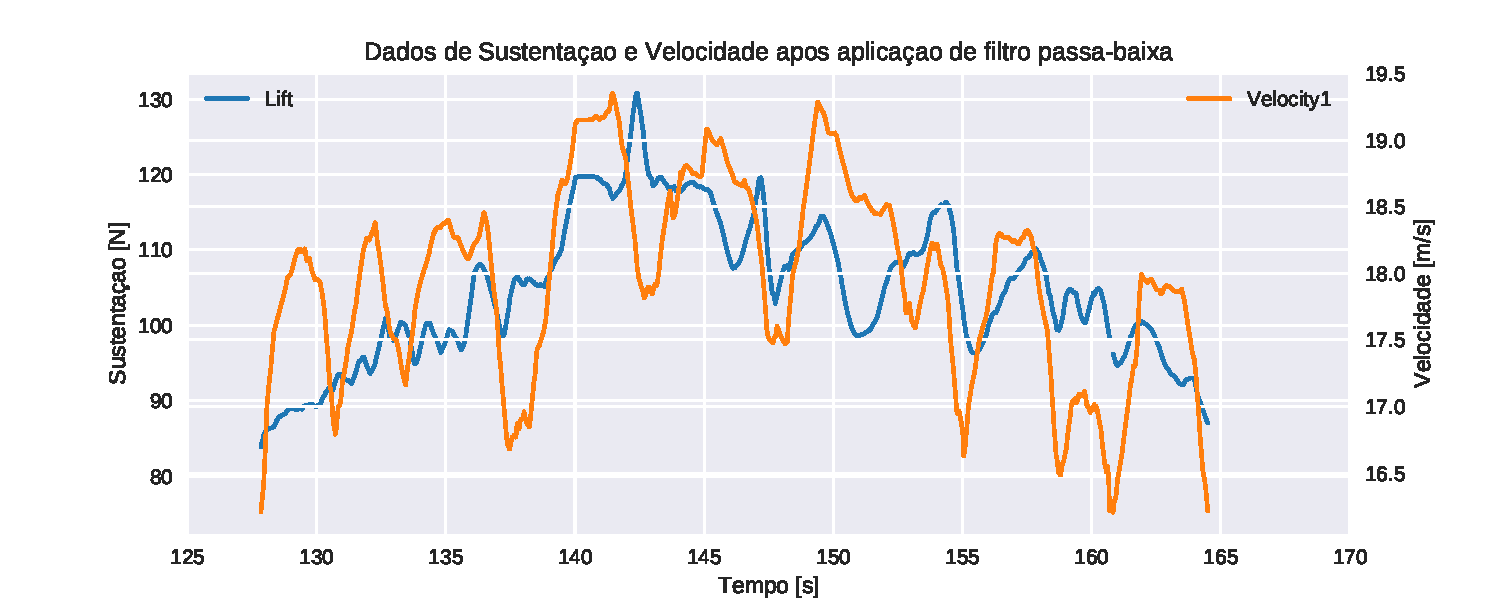
\includegraphics[width=.8\linewidth]{plots/filtered_lift_plot.pdf}
    \caption{DADOS APOS PASSA-BAIXA\cite{autor}.}
    \label{fig:filtered_lift_plot}
\end{figure}

\subsection{Redução}

Em posse dos dados filtrados passa-se a etapa de redução. Não é do interesse do projetista a principio saber qual sustentação, arrasto ou momento foram alcançados durante os testes, pois esses são dados absolutos que dependem do tamanho do componente e da velocidade no instante medido[X]. Para facilidade de analise e mais justa comparação entre diferentes componentes é de interesse a redução destes dados na forma dos coeficientes aerodinâmicos[X].

\begin{equation}
    C_L =  \frac{L}{ \frac{1}{2} \rho V^{2} S} 
\end{equation}

\begin{equation} 
    C_D =  \frac{D}{ \frac{1}{2} \rho V^{2} S}
\end{equation}

\begin{equation}
    C_M =  \frac{M}{ \frac{1}{2} \rho V^{2} S C_{M.A.}} 
\end{equation}

As equações XYZ foram aplicadas a todas as amostras de dados gerando três novas colunas, CL, CD e CM, que podem ser visualizadas na figura \ref{fig:coefficients_plot}. Os dados das baterias de testes foram entao condensados nu mesmo conjunto de dados,para o qual entao foram calculados o valor médio e o desvio padrao de cada coeficiente, para cada angulo de incidencia.

\begin{figure}[!ht]
    \centering
    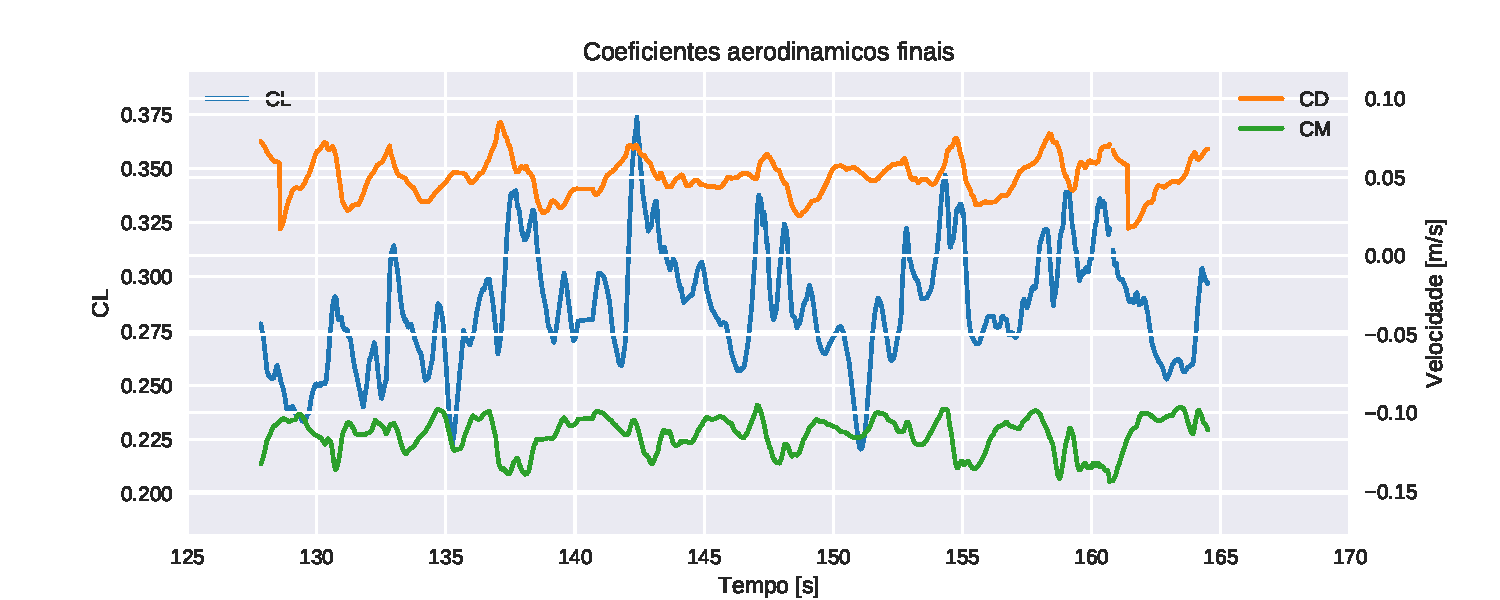
\includegraphics[width=.8\linewidth]{plots/coefficients_plot.pdf}
    \caption{Variação dos coeficientes aerodinâmicos ao longo do tempo para o patamar avaliado\cite{autor}.}
    \label{fig:coefficients_plot}
\end{figure}

Os valores finais de media e desvio padrão para os coeficientes de cada angulo de incidência estão explicitados nos gráficos X Y e Z.

\begin{figure}[!ht]
    \centering
    
\includegraphics[width=.8\linewidth]{figuras/outras/placeholder.png}
    \caption{Curvas $C_x vs Alpha$ com desvio padrao, experimental e simulado.\cite{autor}.}
    \label{fig:coefficients_alpha_plot}
\end{figure}






